\documentclass{article}
\usepackage{amsmath}
\usepackage{amsfonts}
\usepackage[top=1in, bottom=1.25in, left=1.25in, right=1.25in]{geometry}
\usepackage{tikz}

\title{Chapter 1}
\author{Dongie Agnir}
\date{December 8, 2015}

\begin{document}
\maketitle

\section*{1.1 Exercises}
\begin{enumerate}
\item
  \begin{enumerate}
  \item If we let $P$ stand for the statement ``We'll have a reading assignment'' and $Q$ stand for ``We'll have homework problems'' then we can represent the statement as $(P \lor Q) \land \lnot (P \land Q)$.
  \item If we let $P$ stand for the statement ``You will go skiing'' and $Q$ stand for ``There will be snow'', then we can represent the statement as $\lnot P \lor (P \land \lnot Q)$.
    \item $\lnot [(\sqrt{7} < 2) \lor (\sqrt{7} = 2)]$
  \end{enumerate}
\item
  \begin{enumerate}
  \item Let $P$ stand for the statement ``John is telling the truth'' and $Q$ stand for the statement ``Bill is telling the truth'', then we can represent the statement as $(P \land Q) \lor (\lnot P \land \lnot Q)$.
  \item Let the letters $P$, $Q$, and $R$ stand for the statements ``I will have chicken'', ``I will have fish'' and ``I will have mashed potatoes'' respectively, then the statment can be represented as $(P \lor Q) \land \lnot (Q \land R)$.
  \item Let the $P$, $Q$, and $R$ stand for the statements ``$3$ divides $6$'', ``$3$ divides $9$'', and ``$3$ divides $15$'' respectively, then the statement can be represented as $P \land Q \land R$.
  \end{enumerate}
\item For the following, we let $P$ stand for ``Alice is in the room'' and $Q$ stand for ``Bob is in the room''.
  \begin{enumerate}
  \item $\lnot P \lor \lnot Q$
  \item $\lnot P \land \lnot Q$
  \item $\lnot P \lor \lnot Q$
    \item $\lnot P \land \lnot Q$
  \end{enumerate}
\item Only (a) and (c) are well-formed.	 (b) and (c) both contain statements that are not connected by a logical symbol.
\item
  \begin{enumerate}
  \item I will not both buy the pants and not buy the shirt.
  \item I will not buy the pants or shirt.
  \item Either I will not buy the pants, or not buy the shirt.
  \end{enumerate}
\item
  \begin{enumerate}
  \item Either Steve is happy or George is happy, but not both.
  \item Either Steve is happy or George is happy and not Steve, or George is not happy.
  \item Either Steve is happy or George is happy and either Steve or George is not happy.
  \end{enumerate}
\item
  \begin{enumerate}
  \item The \textbf{premise} are: ``Jane and Pete won't both win the math prize'', Pete will win either the math prize or the chemistry prize'', and Jane will win the math prize.''

    The \textbf{conclusion} is ``Therefore, Pete will win the math prize.''

    Let $P$ stand for ``Pete will win the math prize'', $Q$ stand for ``Pete will win the chemistry prize'', and $R$ stand for ``Jane will win the math prize''.

    We can represent the premises in the order given as $\lnot (P \land R)$, $P \lor Q$, and $R$.

    We can represent the conclusion as $Q$.

    Given the premises, yes the conclusion seems reasonable.

  \item The \textbf{premises} are: ``The main course will be either beef or fish.'', ``The vegetable will be either peas or corn.'', and ``We will not have both fish as a main course and corn as a vegetable''.

    The \textbf{conclusion} is ``Therefore we will not have both beef as a main course and peas a vegetable.''

    Let $A$ stand for ``The main course will be beef'', $B$ stand for ``The main course will be fish'', $C$ stand for ``The vegetable will be peas'', and $D$ stand for ``The vegetable will be corn''.

    We can represent the premises as $(A \lor B)$, $(C \lor D)$, and $\lnot (B \land D)$.

    We can represent the conclusion as $\lnot (A \land C)$.

    No, this conclusion does not seem reasonable.  Given the first two premises, there are four possible combinations of main dish and vegetable.  The third premise rules out one of them, but this only concerns fish with peas.

  \item The \textbf{premises} are: ``Either John or Bill is telling the truth.'', ``Either Sam or Bill is lying.''.

    The \textbf{conclusion} is: ``Therefore, either John is telling the truth or Sam is lying.''

    Let $P$ stand for ``John is telling the truth.'', $Q$ stand for ``Bill is telling the truth.'', and $R$ stand for ``Sam is telling the truth.''.

    We can represent the premises as $P \lor Q$ and $\lnot R \lor \lnot Q$.

    We can represent the conclusion as $P \lor \lnot R$.

    Yes, this seems reasonable to me.

  \item
    The \textbf{premise} is ``Either sales will go up and the boss will be happy, or expenses will go up and the boss will be unhappy.''

    The \textbf{conclusion} is ``Sales and expenses will not go up.''

    Let $P$ stand for ``Sales will go up'', $Q$ stand for ``The boss will be happy'', and $R$ stand for ``Expenses will go up''.

    We can represent the premise as $(P \land Q) \lor (R \land \lnot Q)$.

    We can represent the conclusion as $\lnot (P \lor R)$.

    This doesn't seem reasonable because it's possible for $P$ and $Q$ to be true and $R$ to be false, leaving the premise true, and the conclusion false.
    \end{enumerate}
\end{enumerate}

\section*{1.2 Exercises}
\begin{enumerate}
\item
  \begin{enumerate}
  \item
    \begin{tabular}{c c c c}
      $P$ & $Q$ & $\lnot P$ & $\lnot P \lor Q$ \\ \hline
      T & T & F & T \\
      T & F & F & F \\
      F & T & T & T \\
      F & F & T & T \\
    \end{tabular}
  \item
    \begin{tabular}{c c c c c c c}
      $S$ & $G$ & $S \lor G$ & $\lnot S$ & $\lnot G$ & $\lnot S \lor \lnot G$ & $(S \lor G) \land (\lnot S \lor \lnot G)$ \\ \hline
      T & T & T & F & F & F & F \\
      T & F & T & F & T & T & T \\
      F & T & T & T & F & T & T \\
      F & F & F & T & T & T & F \\
    \end{tabular}
  \end{enumerate}
\item
  \begin{enumerate}
  \item
    \begin{tabular}{c c c c c c}
      $P$ & $Q$ & $\lnot P$ & $Q \lor \lnot P$ & $P \land (Q \lor \lnot P)$ & $\lnot [P \land (Q \lor \lnot P)]$ \\ \hline
      T & T & F & T & T & F \\
      T & F & F & F & F & T \\
      F & T & T & T & F & T \\
      F & F & T & T & F & T \\
    \end{tabular}
\item
    \begin{tabular}{c c c c c c c}
      $P$ & $Q$ & $R$ & $P \lor Q$ & $\lnot P$ & $\lnot P \lor R$ & $(P \lor Q) \land (\lnot P \lor R)$ \\ \hline
      T & T & T & T & F & T & T \\
      T & T & F & T & F & F & F \\
      T & F & T & T & F & T & T \\
      T & F & F & T & F & F & F \\
      F & T & T & T & T & T & T \\
      F & T & F & T & T & T & T \\
      F & F & T & F & T & T & F \\
      F & F & F & F & T & T & F \\
      \end{tabular}
  \end{enumerate}
\item
  \begin{enumerate}
  \item
    \begin{tabular}{c c c}
      $P$ & $Q$ & $P + Q$ \\ \hline
      T & T & F \\
      T & F & T \\
      F & T & T \\
      F & F & F \\
    \end{tabular}
  \item $P + Q$ is equivalent to $(\lnot P \land Q) \lor (P \land \lnot Q)$.  This makes intuitive sense because $+$ is true precisely when only either $P$ or $Q$ is true.  Here is the truth table:

    \begin{tabular}{c c c c c c c}
      $P$ & $Q$ & $\lnot P$ & $\lnot Q$ & $\lnot P \land Q$ & $P \land \lnot Q$ & $(\lnot P \land Q) \lor (P \land \lnot Q)$ \\ \hline
      T & T & F & F & F & F & F \\
      T & F & F & T & F & T & T \\
      F & T & T & F & T & F & T \\
      F & F & T & T & F & F & F \\
      \end{tabular}
  \end{enumerate}
\item
  $P \lor Q$ is equivalent to $\lnot (\lnot P \land \lnot Q)$.	Again, this makes intuitive sense because $\lor$ is only false when both $P$ and $Q$ are false.	 We can also think about slightly differently: DeMorgan's law says $\lnot (P \land Q) \equiv \lnot P \lor \lnot Q$, so if we start off by negating both $P$ and $Q$ first we have $\lnot (\lnot P \land \lnot Q) \equiv \lnot\lnot P \lor \lnot\lnot Q \equiv P \lor Q$.  Here is the truth table:

  \begin{tabular}{c c c c c c}
    $P$ & $Q$ & $\lnot P$ & $\lnot Q$ & $\lnot P \land \lnot Q$ & $\lnot (\lnot P \land \lnot Q)$ \\ \hline
    T & T & F & F & F & T \\
    T & F & F & T & F & T \\
    F & T & T & F & F & T \\
    F & F & T & T & T & F \\
  \end{tabular}
\item
  \begin{enumerate}
  \item
    \begin{tabular}{c c c}
      $P$ & $Q$ & $P \downarrow Q$ \\ \hline
      T & T & F \\
      T & F & F \\
      F & T & F \\
      F & F & T \\
      \end{tabular}
      \item
	This truth table shows clearly that it's just the opposite of the one for \textit{or}, so it's equivalent to $\lnot (P \lor Q) \equiv \lnot P \land \lnot Q$.  This makes sense because \textit{nor} should only be true when both $P$ and $Q$ are false.
      \item
	$\lnot P \equiv P \downarrow P$.  This is very useful because we know see that a statement \textit{nor} itself is equivalent to its negation.

	We know that \textit{nor} is the negation of \textit{or}, so if we negate a \textit{nor} then we get a \textit{or}.  Therefore $P \lor Q \equiv \lnot (P \downarrow Q) \equiv (P \downarrow Q) \downarrow (P \downarrow Q)$.  The third equivalence comes directly from our above result.

	$P \downarrow Q \equiv \lnot P \land \lnot Q$, so if we negate $P$ and $Q$ first, we get $\lnot P \downarrow \lnot Q \equiv \lnot \lnot \land P \lnot \lnot Q \equiv P \land Q$.  So, using ony \textit{nor}: $\lnot P \downarrow \lnot Q \equiv (P \downarrow P) \downarrow (Q \downarrow Q) \equiv P \land Q$.
  \end{enumerate}
\item
  \begin{enumerate}
  \item
    \begin{tabular}{c c c}
    $P$ & $Q$ & $(P \uparrow Q)$ \\ \hline
    T & T & F \\
    T & F & T \\
    F & T & T \\
    F & F & T \\
    \end{tabular}
  \item
    $P \uparrow Q \equiv \lnot P \land \lnot Q$.
  \item
    $\lnot P \equiv P \uparrow P$.

    We know $P \uparrow Q \equiv \lnot P \land \lnot Q$, so $\lnot (P \uparrow Q) \equiv \lnot (\lnot P \land \lnot Q) \equiv P \lor Q \equiv (P \uparrow Q) \uparrow (P \uparrow Q)$.

    $P \uparrow Q \equiv \lnot P \land \lnot Q$, so negating $P$ and $Q$ first: $\lnot P \uparrow \lnot Q \equiv \lnot \lnot P \land \lnot \lnot Q \equiv P \land Q \equiv (P \uparrow P) \uparrow (Q \uparrow Q)$.

    Interestingly, these look identical to the results from problem 5.
  \end{enumerate}
  \item
  \begin{enumerate}
  \item
    For this, we determined that the premises are $\lnot (P \land R)$, $P \lor Q$, and $R$, and the conclusion is $Q$.	Here is the truth table:

    \begin{tabular}{c c c c c c}
      $P$ & $Q$ & $R$ & $P \land R$ & $\lnot (P \land R)$ & $P \lor Q$ \\ \hline
      T & T & T & T & F & T \\
      T & T & F & F & T & T \\
      T & F & T & T & F & T \\
      T & F & F & F & T & T \\
      F & T & T & F & T & T \\
      F & T & F & F & T & T \\
      F & F & T & F & T & F \\
      F & F & F & F & T & F \\
    \end{tabular}

    As we can see, all three premises are true on row 5, and so is the conclusion, so this argument is valid.

  \item
    The premises are $(A \lor B)$, $(C \lor D)$, and $\lnot (B \land D)$, and the conclusion is $\lnot (A \land C)$.

    Here is the truth table.  To save time and space, I only have the premises and conclusion.

    \begin{tabular}{c c c c}
      $A \lor B$ & $C \lor D$ & $\lnot (B \land D)$ & $\lnot (A \land C)$ \\ \hline
      T & T & F & F \\
      T & T & T & F \\
      T & T & F & T \\
      T & F & T & T \\
      T & T & T & F \\
      T & T & T & F \\
      T & T & T & T \\
      T & F & T & T \\
      T & T & F & T \\
      T & T & T & T \\
      T & T & F & T \\
      T & F & T & T \\
      F & T & T & T \\
      F & T & T & T \\
      F & T & T & T \\
      F & F & T & T \\
    \end{tabular}

    As we can see, all three premises are true for rows 2, 5, 6, 7, and 10, but of those rows, the conclusion is true only for row 7 and 10.  This argument is invalid.

  \item The premises are $P \lor Q$ and $\lnot R \lor \lnot Q$, and the conclusion is $P \lor \lnot R$.

    Here is the truth table for the premises and conclusion:

    \begin{tabular}{c c c}
      $P \lor Q$ & $\lnot R \lor \lnot Q$ & $P \lor \lnot R$ \\ \hline
      T & F & T \\
      T & T & T \\
      T & T & T \\
      T & T & T \\
      T & F & F \\
      T & T & T \\
      F & T & F \\
      F & T & T \\
    \end{tabular}

    The premises are both true for rows 2, 3, 4, and 6, and for those rows the conclusion is also true so this argument is valid.
  \item
    The premise is $(P \land Q) \lor (R \land \lnot Q)$, and the conclusion is $\lnot P \land \lnot R$.

    Here is the truth table:

    \begin{tabular}{l r}
      $(P \land Q) \lor (R \land \lnot Q)$ & $\lnot (P \land R)$ \\ \hline
      T & F \\
      T & T \\
      T & F \\
      F & T \\
      F & T \\
      F & T \\
      T & T \\
      F & T \\
    \end{tabular}

    The premise is true for rows 1, 2, 3, and 7, but of those rows, the conclusion is true only for rows 2 and 7, so this argument is invalid.
  \end{enumerate}
\item
  The truth table:

  \begin{tabular}{c c c c c c c}
    $P$ & $Q$ & $(P \land Q) \lor (\lnot P \land \lnot Q)$ & $\lnot P \lor Q$ & $(P \lor \lnot Q) \land (Q \lor \lnot P)$ & $\lnot(P \lor Q)$ & $(Q \land P) \lor \lnot P$ \\ \hline
    T & T & T & T & T & F & T \\
    T & F & F & F & F & F & F \\
    F & T & F & T & F & F & T \\
    F & F & T & T & T & T & T \\
  \end{tabular}

  Looking at the table, we can see that $(P \land Q) \lor (\lnot P \land \lnot Q) \equiv (P \lor \lnot Q) \land (Q \lor \lnot P)$, and $\lnot P \lor Q \equiv (Q \land P) \lor \lnot P$.
\item
  The truth tables:

  \begin{tabular}{c c c c c}
    $P$ & $Q$ & $(P \lor Q) \land (\lnot P \lor \lnot Q)$ & $(P \lor Q) \land (\lnot P \land \lnot Q)$ & $(P \lor Q) \lor (\lnot P \lor \lnot Q)$ \\ \hline
    T & T & F & F & T \\
    T & F & T & F & T \\
    F & T & T & F & T \\
    F & F & F & F & T \\
  \end{tabular}

  \begin {tabular}{c c c c}
    $P$ & $Q$ & $R$ & $[P \land (Q \lor \lnot R)] \lor (\lnot P \lor R)$ \\ \hline
    T & T & T & T \\
    T & T & F & T \\
    T & F & T & T \\
    T & F & F & T \\
    F & T & T & T \\
    F & T & F & T \\
    F & F & T & T \\
    F & F & F & T \\
  \end{tabular}

  We can see that (a) is neither, (b) is a contradiction, and (c) and (d) are tautologies.

\item
  \begin{enumerate}
  \item

    \begin{tabular}{c c c c c c c}
      $P$ & $Q$ & $(P \lor Q)$ & $\lnot (P \lor Q)$ & $\lnot P$ & $\lnot Q$ & $\lnot P \land \lnot Q$ \\ \hline
      T & T & T & F & F & F & F \\
      T & F & T & F & F & T & F \\
      F & T & T & F & T & F & F \\
      F & F & F & T & T & T & T \\
    \end{tabular}
  \item
    The first distributive law: $P \land (Q \lor R) \equiv (P \land Q) \lor (P \land R)$.

    \begin{tabular}{c c c c c}
      $P$ & $Q$ & $R$ & $(Q \lor R)$ & $P \land (Q \lor R)$ \\ \hline
      T & T & T & T & T \\
      T & T & F & T & T \\
      T & F & T & T & T \\
      T & F & F & F & F \\
      F & T & T & T & F \\
      F & T & F & T & F \\
      F & F & T & T & F \\
      F & F & F & F & F \\
    \end{tabular}

    \begin{tabular}{c c c}
      $(P \land Q)$ & $(P \land R)$ & $(P \land Q) \lor (P \land R)$ \\ \hline
      T & T & T \\
      T & F & T \\
      F & T & T \\
      F & F & F \\
      F & F & F \\
      F & F & F \\
      F & F & F \\
      F & F & F \\
    \end{tabular}

    The second distributive law: $P \lor (Q \land R) \equiv (P \lor Q) \land (P \lor R)$.


    \begin{tabular}{c c c c c}
      $P$ & $Q$ & $R$ & $(Q \land R)$ & $P \lor (Q \land R)$ \\ \hline
      T & T & T & T & T \\
      T & T & F & F & T \\
      T & F & T & F & T \\
      T & F & F & F & T \\
      F & T & T & T & T \\
      F & T & F & F & F \\
      F & F & T & F & F \\
      F & F & F & F & F \\
    \end{tabular}

    \begin{tabular}{c c c}
      $P \lor Q$ & $P \lor R$ & $(P \lor Q) \land (P \lor Q)$ \\ \hline
      T & T & T \\
      T & T & T \\
      T & T & T \\
      T & T & T \\
      T & T & T \\
      T & F & F \\
      F & T & F \\
      F & F & F \\
      \end{tabular}
    \end{enumerate}
\item
  \begin{enumerate}
  \item

    \begin{equation*}
      \begin{aligned}
	\lnot (\lnot P \land \lnot Q) & \equiv \lnot \lnot P \lor \lnot \lnot Q && \text{DeMorgan's Law} \\
	& \equiv P \lor Q && \text{double negation law} \\
	\end{aligned}
    \end{equation*}

  \item
    \begin{equation*}
      \begin{aligned}
	(P \land Q) \lor (P \land \lnot Q) & \equiv P \land (Q \lor \lnot Q) && \text{Distributive law} \\
	& \equiv P \land (\text{tautology}) \\
	& \equiv P && \text{tautology laws} \\
	\end{aligned}
    \end{equation*}

  \item
    \begin{equation*}
      \begin{aligned}
	\lnot (P \land \lnot Q) \lor (\lnot P \land Q) & \equiv (\lnot P \lor Q) \lor (\lnot P \land Q) && \text{DeMorgan's law} \\
	& \equiv [(\lnot P \lor Q) \lor \lnot P] \land [(\lnot P \lor Q) \lor Q] && \text{Distributive law} \\
	& \equiv [(\lnot P \lor \lnot P) \lor Q] \land [\lnot P \lor (Q \lor Q)] && \text{Associative law and Commutative law} \\
	& \equiv (\lnot P \lor Q) \land (\lnot P \lor Q) && \text{Idempotent laws} \\
	& \equiv \lnot P \lor Q && \text{Idempotent laws} \\
	\end{aligned}
    \end{equation*}
  \end{enumerate}
\item
  TODO.
\item
  The Double negation law says that negating a negation cancels it out, so
  \begin{equation*}
    \lnot P \land \lnot Q \equiv \lnot \lnot (\lnot P \land \lnot Q)
  \end{equation*}

  Using the first DeMorgan's law, we can negate the statement within the parenthesis:

  \begin{equation*}
    \begin{aligned}
      \lnot \lnot (\lnot P \land \lnot Q) & \equiv \lnot (\lnot \lnot P \lor \lnot \lnot Q) \\
      & \equiv \lnot (P \lor Q) \\
      \end{aligned}
  \end{equation*}

  Therefore, we've shown that $\lnot (P \lor Q) \equiv \lnot P \land \lnot Q$.

\item
  \begin{equation*}
    \begin{aligned}
      (P \land (Q \land R)) \land S & \equiv ((P \land Q) \land R) \land S \\
      & \equiv (P \land Q) \land (R \land S) \\
    \end{aligned}
  \end{equation*}

\item Each letter can have two values, true or false.  Each line in a truth table corresponds to a unique combination of the possible values for each letter.  Therefore, there are $2^n$ lines for $n$ letters.

\item From looking at the values, a good guess is that this involves $\lor$ because it's false only once.  Since the first line where both values are false is true, then that signals that one or both of them is negated, and the second line, where $P$ is false and $Q$ is true, and the formula is false suggests that it's $Q$ that's negated, so my guess is the formula is $P \lor \lnot Q$.  Here is the truth table:

  \begin{tabular}{c c c c}
    $P$ & $Q$ & $\lnot Q$ & $P \lor \lnot Q$ \\ \hline
    F & F & T & T \\
    F & T & F & F \\
    T & F & T & T \\
    T & T & F & T \\
    \end{tabular}

\item This is just the truth table for \textit{exclusive or} which we know from problem 3 is equivalent to $(P \land \lnot Q) \lor (\lnot P \land Q)$.

\item To be valid, the premises cannot all be true without the conclusion being true as well.  So, if the conclusion is a tautology, then argument is valid, since whenever the premises are true (including never), we know that the conclusion is true as well.  If the conclusion is a contradiction, then the premises must also be a contradiction to be a valid argument.	 If the premises are a tautology, then the conclusion must also be a tautology to be valid.  If the premises are a contradiction, then argument is always valid.
\end{enumerate}
\section*{1.3 Exercises}
\begin{enumerate}
\item
  \begin{enumerate}
  \item
    Let $D(x, y)$ stand for ``$x$ divides $y$'', then we can represent the statement as $D(3,6) \land D(3,9) \land D(3,15)$.
  \item
    Using the definition of $D(x, y)$ from above, $D(2,x) \land D(3,x) \land \lnot D(4,x)$.
  \item
    Let $P(x)$ stand for ``$x$ is prime''.  $x \in \mathbb{N} \land y \in \mathbb{N} \land [(\lnot P(x) \land P(y)) \lor (P(x) \land \lnot P(y))]$.
  \end{enumerate}
\item
  \begin{enumerate}
    \item
      Let $M(x)$ stand for ``$x$ is a man'', and $T(x,y)$ stand for ``$x$ is taller than $y$''.	 $M(x) \land M(y) \land (T(x,y) \lor T(y,x))$.
    \item
      Let $B(x)$ stand for ``$x$ has brown eyes'', and $R(x)$ stand for ``$x$ has red hair''.  $(B(x) \lor B(y)) \land (R(x) \lor R(y))$.
    \item
      Using the same definitions as above, $(B(x) \land R(x)) \lor (B(y) \land R(y))$.

  \end{enumerate}
\item
  \begin{enumerate}
  \item
    $\{x | x \text{ is a planet in our solar system}\}$.
  \item
    $\{x | x \text{ is part of the Ivy League}\}$.
  \item
    $\{x | x \text{ is a U.S. State}\}$.
  \item
    $\{x | x \text{ is a Canadian province}\}$.
  \end{enumerate}
\item
  \begin{enumerate}
  \item
    $\{x^{2} | x \in \mathbb{N}^{+}\}$
  \item
    $\{2^{x} | x \in \mathbb{N}\}$
  \item
    $\{x \in \mathbb{N} | 9 < x < 20\}$.

  \end{enumerate}
\item
  \begin{enumerate}
  \item
    \begin{equation*}
      -3 \in \{x \in \mathbb{R} | 13 - 2x > 1\} \equiv -3 \in \mathbb{R} \land 13 - 2(-3) > 1
    \end{equation*}
    $x$ is a bound variable and there are no free variables; this statement is true.
  \item
    \begin{equation*}
      4 \in \{x \in \mathbb{R}^{-} | 13 - 2x > 1\} \equiv 4 \in \mathbb{R}^{-} \land 13 - 2(4) > 1
    \end{equation*}
    $x$ is a bound variable and there are no free variables; this statement is false; in particular, $4 \in \mathbb{R}^{-}$ is false because 4 is not a negative real number.
    \item
  \begin{equation*}
    5 \notin \{x \in \mathbb{R} | 13 - 2x > c\} \equiv \lnot(5 \in \mathbb{R} \land 13 - 2(5) > c)
  \end{equation*}
  $x$ is a bound variable and $c$ is free variable.
  \end{enumerate}
\item
  \begin{enumerate}
  \item
    \begin{equation*}
      w \in \{x \in \mathbb{R} | 13 - 2x > c\} \equiv (w \in \mathbb{R}) \land (13 -2w > c)
    \end{equation*}
    $x$ is a bound variable, and $w$ and $c$ are free variables.
  \item
    \begin{equation*}
      4 \in \{x \in \mathbb{R} | 13 - 2x \in \{ y | y \text{ is a prime number}\} \} \equiv (4 \in \mathbb{R}) \land P(13 - 2(4))
    \end{equation*}
    where $P(x)$ stands for ``$x$ is a prime number''.

    $x$ and $y$ are bound variables and there are no free variables.  This statement is true.
  \item
    \begin{equation*}
      4 \in \{x \in \{y | y \text{ is a prime number}\} | 13 -2x > 1\} \equiv P(4) \land (13 - 2(4) > 1)
    \end{equation*}
    where $P(x)$ stands for ``$x$ is a prime number''.

    $x$ and $y$ are bound variables and there are not free variables.  This statement is false.
  \end{enumerate}
\item
  \begin{enumerate}
  \item
    \begin{equation*}
      \begin{aligned}
	\{ \text{Conrad Hilton, Jr.}, \text{Michael Wilding}, \text{Mike Todd}, \\
	\text{Eddie Fisher}, \text{Richard Burton}, \text{John Warner}, \text{Larry Fortensky}
      \}
      \end{aligned}
    \end{equation*}
  \item
    $\{\land, \lor, \lnot, +, \uparrow, | \}$
  \item
    $\{\text{Daniel J. Velleman}\}$
  \end{enumerate}
\item
  \begin{enumerate}
  \item $\{1, 3\}$
  \item $\{\}$
  \item $\{x \in \mathbb{R} | -5 < x < 5\}$
  \end{enumerate}
\end{enumerate}
\section*{1.4 Exercises}
\begin{enumerate}
\item
  For the following problems, $A = \{1,3,12,35\}$, $B = \{3,7,12,20\}$, and $C = \{x \mid x \text{ is a prime number}\}$.
  \begin{enumerate}
  \item
    $A \cap B = \{3,12\}$
  \item
    $(A \cup B) \setminus C = \{1,3,7,12,20,35\} \setminus C = \{1,12,20,35\}$
  \item
    $A \cup (B \setminus C) = A \cup \{12, 20\} = \{1,3,12,20,35\}$.
  \end{enumerate}
  None of the sets are disjoint from any other set.  We can see that $((A \cup B) \setminus C) \subseteq (A \cup (B \setminus C))$ and $(A \cap B) \subseteq (A \cup (B \setminus C))$.
\item
  For the following, $A = \{\text{United States}, \text{Germany}, \text{China}, \text{Australia}\}, B = \{\text{Germany}, \text{France}, \text{India}, \text{Brazil}\}, C = \{x \mid x \text{ is a country in Europe}\}$.
  \begin{enumerate}
  \item
    $A \cap B = \{\text{Germany}\}$
  \item
    \begin{equation*}
      \begin{aligned}
	(A \cup B) \setminus C &= \{\text{United States}, \text{Germany}, \text{China}, \text{Australia}, \text{France}, \text{India}, \text{Brazil}\} \setminus C \\
	&= \{\text{United States}, \text{China}, \text{Australia}, \text{India}, \text{Brazil}\}
       \end{aligned}
    \end{equation*}
  \item
    \begin{equation*}
      \begin{aligned}
	(B \cap C) \setminus A &= \{\text{Germany}, \text{France}\} \setminus A \\
	&= \{\text{France}\}
      \end{aligned}
      \end{equation*}
  \end{enumerate}
\item Below is the Venn diagram corresponding to $A \cap B$:

  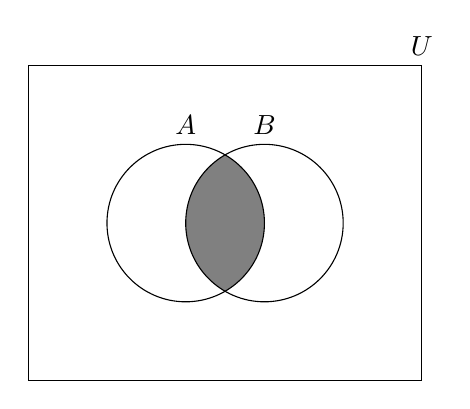
\begin{tikzpicture}[fill=gray]
    \scope
    \clip (1,0) circle (1);
    \fill (0,0) circle (1);
    \endscope
    \draw (0,0) circle (1) (0,1) node [text=black,above] {$A$};
    \draw (1,0) circle (1) (1,1) node [text=black,above] {$B$};
    \draw (-2,-2) rectangle (3,2) node [text=black,above] {$U$};
  \end{tikzpicture}

  \pagebreak
  and also the Venn diagram for $A \cup B$:

  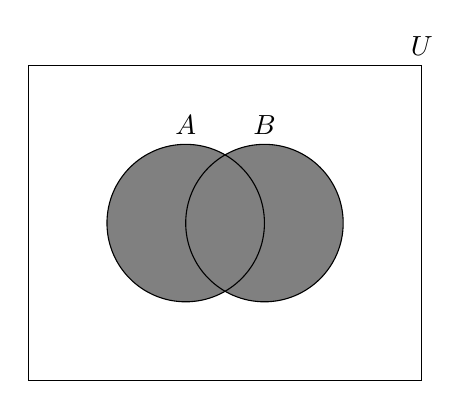
\begin{tikzpicture}[fill=gray]
    \scope
    \clip (-2,-2) rectangle (2,2);
    \fill (0,0) circle (1);
    \fill (1,0) circle (1);
    \endscope
    \draw (0,0) circle (1) (0,1) node [text=black,above] {$A$};
    \draw (1,0) circle (1) (1,1) node [text=black,above] {$B$};
    \draw (-2,-2) rectangle (3,2) node [text=black,above] {$U$};
  \end{tikzpicture}

  Going back to the definition of $A \setminus B$, we see that the elements in $A \cup B$ that are not in $A \cap B$ are exactly where $A$ and $B$ don't overlap, and so we remove the overlapping part giving us:

  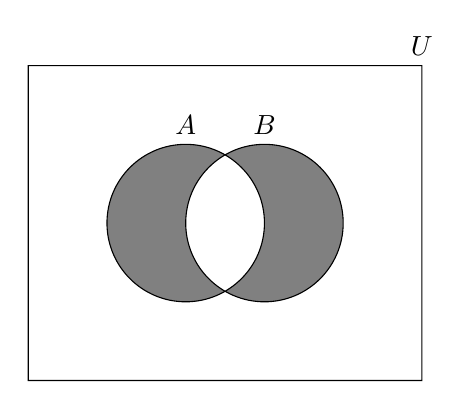
\begin{tikzpicture}[fill=gray]
    \scope
    \clip (-2,-2) rectangle (2,2) (1,0) circle (1);
    \fill (0,0) circle (1);
    \endscope
    \scope
    \clip (-2,-2) rectangle (2,2) (0,0) circle (1);
    \fill (1,0) circle (1);
    \endscope
    \draw (-2,-2) rectangle (3,2) node [text=black,above] {$U$}
    (0,0) circle (1) (0, 1) node [text=black,above] {$A$}
    (1,0) circle (1) (1, 1) node [text=black,above] {$B$};
  \end{tikzpicture}

  Here is the Venn diagram for $A \setminus B$.	 The elements of the set are elements of $A$ that are not also in $B$, so we need to exclude the area where they overlap.

  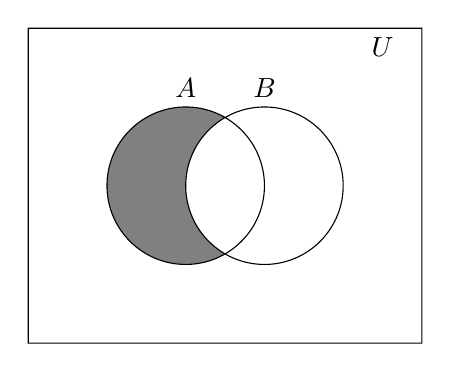
\begin{tikzpicture}[fill=gray]
    \scope
    \clip (-2,-2) rectangle (2,2) (1,0) circle (1);
    \fill (0,0) circle (1);
    \endscope
    \draw (-2,-2) rectangle (3,2) (2.5,2) node [text=black,below] {$U$}
    (0,0) circle (1) (0,1) node [text=black,above] {$A$}
    (1,0) circle (1) (1,1) node [text=black,above] {$B$};
  \end{tikzpicture}

  It's a similar diagram for $B \setminus A$:

  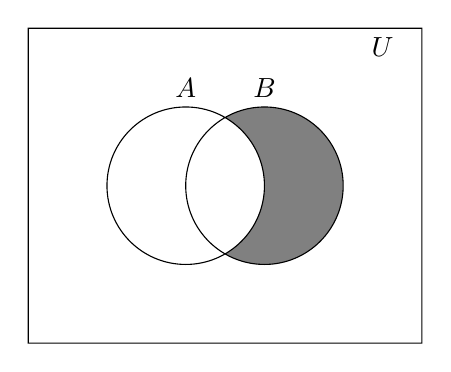
\begin{tikzpicture}[fill=gray]
    \scope
    \clip (-2,-2) rectangle (2,2) (0,0) circle (1);
    \fill (1,0) circle (1);
    \endscope
    \draw (-2,-2) rectangle (3,2) (2.5,2) node [text=black,below] {$U$}
    (0,0) circle (1) (0,1) node [text=black,above] {$A$}
    (1,0) circle (1) (1,1) node [text=black,above] {$B$};
  \end{tikzpicture}

  $(A \setminus B) \cup (B \setminus A)$ just combines the elements of both sets, and so again we end up with the same diagram as Figure 5.

\item
  \begin{enumerate}
    \item
  $A \cap B$ is where $A$ and $B$ overlap:

  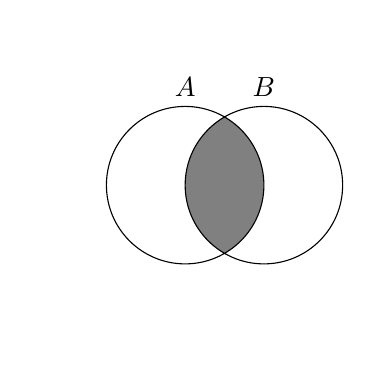
\begin{tikzpicture}[fill=gray]
    \fill (1,0) circle (1);
    \scope
    \clip (-2,-2) rectangle (2,2) (0,0) circle (1);
    \fill[fill=white] (1,0) circle (1);
    \endscope
    \draw (0,0) circle (1) (0,1) node [text=black,above] {$A$}
    (1,0) circle (1) (1,1) node [text=black,above] {$B$};
  \end{tikzpicture}

  Note that $(A \cap B) \subset B$; and of course just $A$ is:

  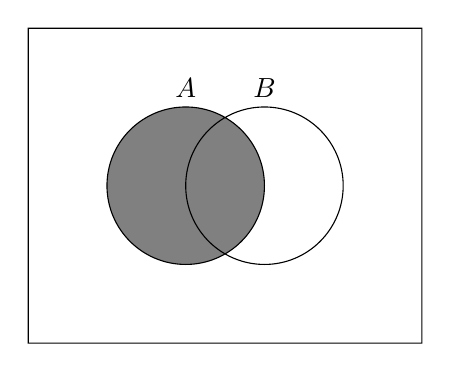
\begin{tikzpicture}[fill=gray]
        \fill (0,0) circle (1);
    \draw (0,0) circle (1) (0,1) node [text=black,above] {$A$}
    (1,0) circle (1) (1,1) node [text=black,above] {$B$}
    (-2,-2) rectangle (3,2);

  \end{tikzpicture}

  Again, going back to the definition of set difference, it's all th elements of $A$ that are not also in $A \cap B$:

  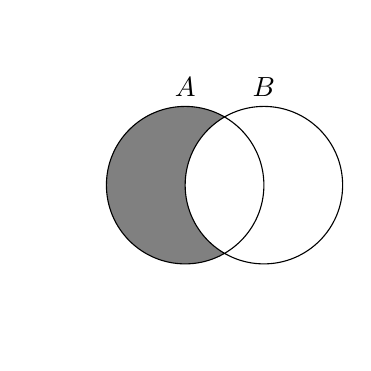
\begin{tikzpicture}[fill=gray]
    \scope
    \clip (-2,-2) rectangle (2,2) (1,0) circle (1);
    \fill (0,0) circle (1);
    \endscope
    \draw (0,0) circle (1) (0,1) node [text=black,above] {$A$}
    (1,0) circle (1) (1,1) node [text=black,above] {$B$};
  \end{tikzpicture}

  \pagebreak

  This is exactly the same as $A \setminus B$ since $A$ is:

  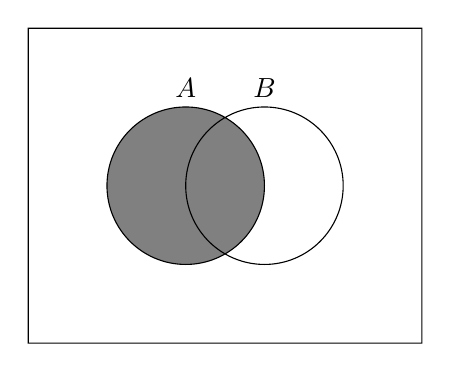
\begin{tikzpicture}[fill=gray]
        \fill (0,0) circle (1);
    \draw (0,0) circle (1) (0,1) node [text=black,above] {$A$}
    (1,0) circle (1) (1,1) node [text=black,above] {$B$}
    (-2,-2) rectangle (3,2);

    \end{tikzpicture}

    $B$ is:

    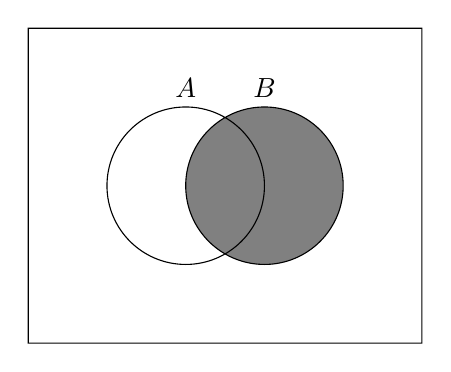
\begin{tikzpicture}[fill=gray]
          \fill (1,0) circle (1);
    \draw (0,0) circle (1) (0,1) node [text=black,above] {$A$}
    (1,0) circle (1) (1,1) node [text=black,above] {$B$}
    (-2,-2) rectangle (3,2);

    \end{tikzpicture}


  And so, all the elements of $A$ that are also not in $B$ looks exactly like the diagram for $A \setminus (A \cap B)$.
\item
  $A$ looks like the following:

  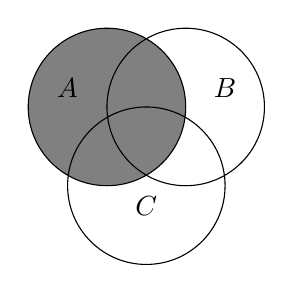
\begin{tikzpicture}[fill=gray]
    \fill (0,0) circle (1);
    \draw (0,0) circle (1) (-0.5,0) node [text=black,above] {$A$}
    (1,0) circle (1) (1.5, 0) node [text=black,above] {$B$}
    (0.5,-1) circle (1) (0.5,-1.5) node [text=black,above] {$C$};
  \end{tikzpicture}

  and $B \cap C$:

  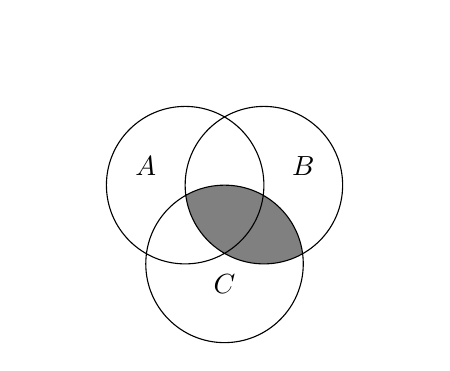
\begin{tikzpicture}[fill=gray]
    \fill (0.5,-1) circle (1)
    (1,0) circle (1);

    \scope
    \clip (-2,-2) rectangle (3,2) (1,0) circle (1);
    \fill[fill=white] (0.5,-1) circle (1);
    \endscope

    \scope
    \clip (-2,-2) rectangle (3,2) (0.5,-1) circle (1);
    \fill[fill=white] (1,0) circle (1);
    \endscope


    \draw (0,0) circle (1) (-0.5,0) node [text=black,above] {$A$}
    (1,0) circle (1) (1.5, 0) node [text=black,above] {$B$}
    (0.5,-1) circle (1) (0.5,-1.5) node [text=black,above] {$C$};
  \end{tikzpicture}

  \pagebreak
  and the union of the two, $A \cup (B \cap C)$, is simply:

  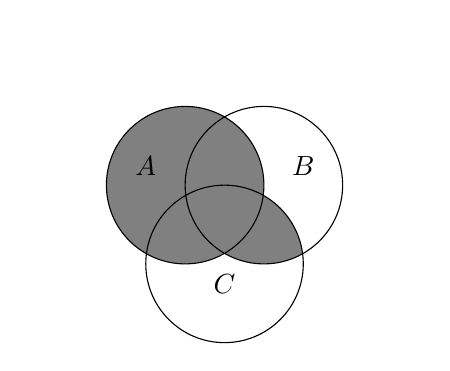
\begin{tikzpicture}[fill=gray]
    \fill (0.5,-1) circle (1)
    (1,0) circle (1);

    \scope
    \clip (-2,-2) rectangle (3,2) (1,0) circle (1);
    \fill[fill=white] (0.5,-1) circle (1);
    \endscope

    \scope
    \clip (-2,-2) rectangle (3,2) (0.5,-1) circle (1);
    \fill[fill=white] (1,0) circle (1);
    \endscope

    \fill (0,0) circle (1);

    \draw (0,0) circle (1) (-0.5,0) node [text=black,above] {$A$}
    (1,0) circle (1) (1.5, 0) node [text=black,above] {$B$}
    (0.5,-1) circle (1) (0.5,-1.5) node [text=black,above] {$C$};
  \end{tikzpicture}

    The diagram for $A \cup B$:

  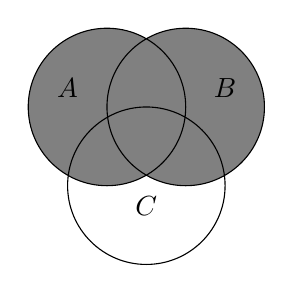
\begin{tikzpicture}[fill=gray]
    \fill (0,0) circle (1)
    (1,0) circle (1);

    \draw (0,0) circle (1) (-0.5,0) node [text=black,above] {$A$}
    (1,0) circle (1) (1.5, 0) node [text=black,above] {$B$}
    (0.5,-1) circle (1) (0.5,-1.5) node [text=black,above] {$C$};
  \end{tikzpicture}

    and for $A \cup C$:

  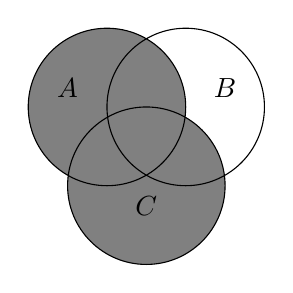
\begin{tikzpicture}[fill=gray]
    \fill (0,0) circle (1)
    (0.5,-1) circle (1);

    \draw (0,0) circle (1) (-0.5,0) node [text=black,above] {$A$}
    (1,0) circle (1) (1.5, 0) node [text=black,above] {$B$}
    (0.5,-1) circle (1) (0.5,-1.5) node [text=black,above] {$C$};
  \end{tikzpicture}

  It's easy to see that the union of the two is all of $A$ as well as the elements $B$ and $C$ share, resulting the same diagram as $A \cup (B \cap C)$.
  \end{enumerate}
\item
  \begin{enumerate}
  \item
    \begin{equation*}
      \begin{aligned}
	x \in A \setminus (A \cap B) &\equiv (x \in A) \land x \notin (A \cap B) & \text{Def. of set difference} \\
	&\equiv (x \in A) \land ((x \notin A) \lor (x \notin B)) & \text{Def. of set intersect}\\
	&\equiv (x \in A \land x \notin A) \lor (x \in A \land x \notin B) & \text{Distrubutive rule}\\
	&\equiv F \lor (x \in A \land x \notin B) & \text{Tautology}\\
	&\equiv (x \in A \land x \notin B) \\
	&\equiv A \setminus B
      \end{aligned}
    \end{equation*}
  \item
    \begin{equation*}
      \begin{aligned}
        x \in A \cup (B \cap C) &\equiv x \in A \lor x \in (B \cap C) & \text{Def. of set union} \\
        &\equiv x \in A \lor (x \in B \land x \in C) & \text{Def of set intersect}\\
        &\equiv (x \in A \lor x \in B) \land (x \in A \lor x \in C) & \text{Distributive rule}\\
        &\equiv x \in (A \cup B) \land x \in (A \cup C) & \text{Def. of set union} \\
        &\equiv x \in (A \cup B) \cap (A \cup C) & \text{Def. of set intersect}
        \end{aligned}
      \end{equation*}
  \end{enumerate}
  \pagebreak
\item
  \begin{enumerate}
    \item
  $(A \cup B) \setminus C = (A \setminus C) \cup (B \setminus C)$

  The diagrams for $A \cup B$, and $C$:

  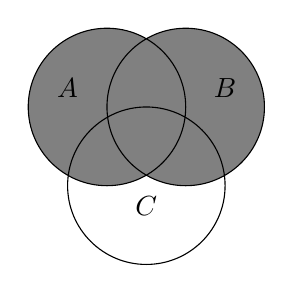
\begin{tikzpicture}[fill=gray]
    \fill (0,0) circle (1)
    (1,0) circle (1);

    \draw (0,0) circle (1) (-0.5,0) node [text=black,above] {$A$}
    (1,0) circle (1) (1.5, 0) node [text=black,above] {$B$}
    (0.5,-1) circle (1) (0.5,-1.5) node [text=black,above] {$C$};
  \end{tikzpicture}
    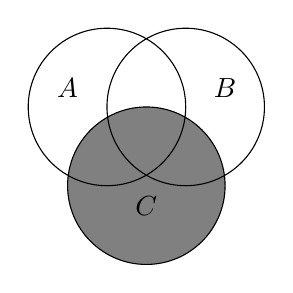
\begin{tikzpicture}[fill=gray]
    \fill (0.5,-1) circle (1);

    \draw (0,0) circle (1) (-0.5,0) node [text=black,above] {$A$}
    (1,0) circle (1) (1.5, 0) node [text=black,above] {$B$}
    (0.5,-1) circle (1) (0.5,-1.5) node [text=black,above] {$C$};
    \end{tikzpicture}

    We remove everything in $C$ from $A \cup B$ leaving:

    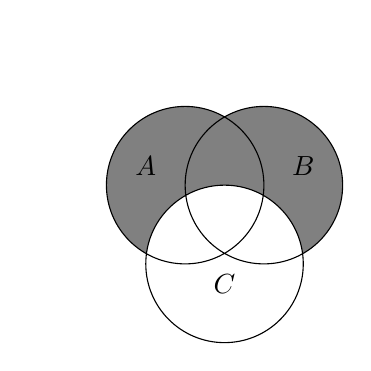
\begin{tikzpicture}[fill=gray]
      \scope
      \clip (-2,-2) rectangle (2,2)
      (0.5,-1) circle (1);
      \fill (0,0) circle (1)
      (1,0) circle (1);
      \endscope

    \draw (0,0) circle (1) (-0.5,0) node [text=black,above] {$A$}
    (1,0) circle (1) (1.5, 0) node [text=black,above] {$B$}
    (0.5,-1) circle (1) (0.5,-1.5) node [text=black,above] {$C$};
    \end{tikzpicture}

    The diagrams for $A \setminus C$ and $B \setminus C$:

    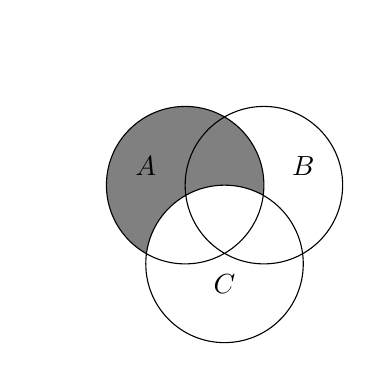
\begin{tikzpicture}[fill=gray]
      \scope
      \clip (0.5,-1) circle (1)
      (-2,-2) rectangle (2,2);
      \fill (0,0) circle (1);
      \endscope

    \draw (0,0) circle (1) (-0.5,0) node [text=black,above] {$A$}
    (1,0) circle (1) (1.5, 0) node [text=black,above] {$B$}
    (0.5,-1) circle (1) (0.5,-1.5) node [text=black,above] {$C$};
    \end{tikzpicture}
    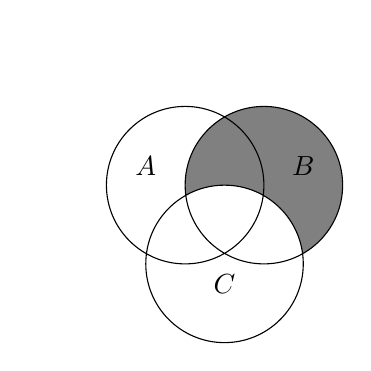
\begin{tikzpicture}[fill=gray]
      \scope
      \clip (0.5,-1) circle (1)
      (-2,-2) rectangle (2,2);
      \fill (1,0) circle (1);
      \endscope

    \draw (0,0) circle (1) (-0.5,0) node [text=black,above] {$A$}
    (1,0) circle (1) (1.5, 0) node [text=black,above] {$B$}
    (0.5,-1) circle (1) (0.5,-1.5) node [text=black,above] {$C$};
    \end{tikzpicture}

    Combining all the shaded areas gives us the same result as above.
  \item
    $A \cup (B \setminus C) = (A \cup B) \setminus (C \setminus A)$

    The diagram for $A$ and $B \setminus C$:

    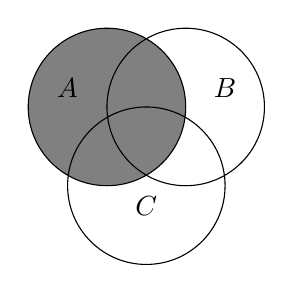
\begin{tikzpicture}[fill=gray]
      \fill (0,0) circle (1);
    \draw (0,0) circle (1) (-0.5,0) node [text=black,above] {$A$}
    (1,0) circle (1) (1.5, 0) node [text=black,above] {$B$}
    (0.5,-1) circle (1) (0.5,-1.5) node [text=black,above] {$C$};
    \end{tikzpicture}
    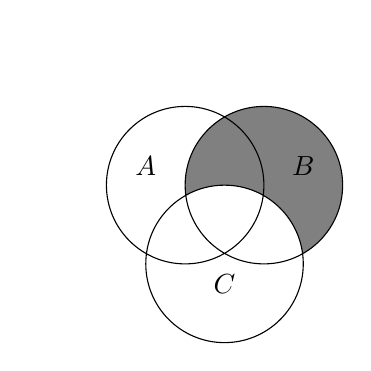
\begin{tikzpicture}[fill=gray]
      \scope
      \clip (0.5,-1) circle (1)
      (-2,-2) rectangle (2,2);
      \fill (1,0) circle (1);
      \endscope

    \draw (0,0) circle (1) (-0.5,0) node [text=black,above] {$A$}
    (1,0) circle (1) (1.5, 0) node [text=black,above] {$B$}
    (0.5,-1) circle (1) (0.5,-1.5) node [text=black,above] {$C$};
    \end{tikzpicture}

    \pagebreak
    Combining the shaded parts:

    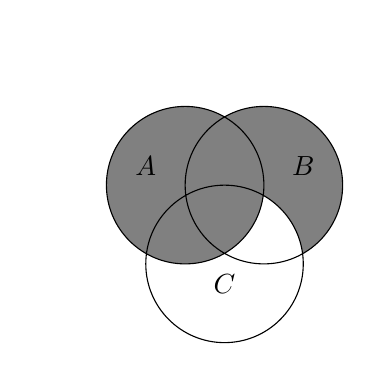
\begin{tikzpicture}[fill=gray]
      \scope
      \clip (0.5,-1) circle (1)
      (-2,-2) rectangle (2,2);
      \fill (1,0) circle (1);
      \endscope
      \fill (0,0) circle (1);


    \draw (0,0) circle (1) (-0.5,0) node [text=black,above] {$A$}
    (1,0) circle (1) (1.5, 0) node [text=black,above] {$B$}
    (0.5,-1) circle (1) (0.5,-1.5) node [text=black,above] {$C$};
    \end{tikzpicture}

    The diagram for $A \cup B$ and $C \setminus A$:

    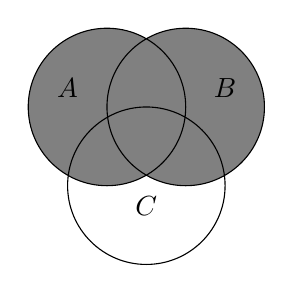
\begin{tikzpicture}[fill=gray]
      \fill (0,0) circle (1)
      (1,0) circle (1);

    \draw (0,0) circle (1) (-0.5,0) node [text=black,above] {$A$}
    (1,0) circle (1) (1.5, 0) node [text=black,above] {$B$}
    (0.5,-1) circle (1) (0.5,-1.5) node [text=black,above] {$C$};
    \end{tikzpicture}
    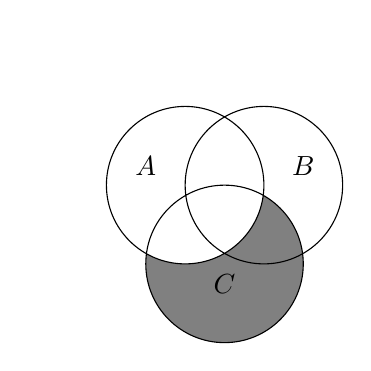
\begin{tikzpicture}[fill=gray]
      \scope
      \clip (0,0) circle (1)
      (-2,-2) rectangle (2,2);
      \fill (0.5,-1) circle (1);
      \endscope
    \draw (0,0) circle (1) (-0.5,0) node [text=black,above] {$A$}
    (1,0) circle (1) (1.5, 0) node [text=black,above] {$B$}
    (0.5,-1) circle (1) (0.5,-1.5) node [text=black,above] {$C$};
    \end{tikzpicture}

    Removing the shaded regions in the second diagram from the first gives us the same diagram as above.
  \end{enumerate}
\item
  \begin{enumerate}
  \item
    \begin{equation*}
      \begin{aligned}
        x \in (A \cup B) \setminus C &\equiv x \in A \cup B \land x \notin C & \text{Def. of set difference} \\
        &\equiv (x \in A \lor x \in B) \land x \notin C & \text{Def. of set union} \\
        &\equiv (x \in A \land x \notin C) \lor (x \in B \land x \notin C) & \text{Distributive law} \\
        &\equiv x \in (A \setminus C) \lor x \in (B \setminus C) & \text{Def. of set difference} \\
        &\equiv x \in (A \setminus C) \cup (B \setminus C) & \text{Def. of set union}
      \end{aligned}
    \end{equation*}
  \item
    \begin{equation*}
      \begin{aligned}
        x \in A \cup (B \setminus C) &\equiv x \in A \lor x \in (B \setminus C) & \text{Def. of set union}\\
        &\equiv x \in A \lor (x \in B \land x \notin C) & \text{Def. of set difference}\\
        &\equiv (x \in A \lor x \in B) \land (x \in A \lor x \notin C) & \text{Distributive law}\\
        &\equiv (x \in A \lor x \in B) \land \lnot (x \notin A \land x \in C) & \text{DeMorgan's law}\\
        &\equiv x \in (A \cup B) \land x \notin (C \setminus A) & \text{Set union, difference}\\
        &\equiv x \in (A \cup B) \setminus(C \setminus A) & \text{Def. of set difference}
        \end{aligned}
      \end{equation*}
  \end{enumerate}
\item
  \begin{enumerate}
  \item
    \begin{equation*}
      \begin{aligned}
    x \in (A \setminus B) \setminus C &\equiv x \in (A \setminus B) \land x \notin C \\
    &\equiv (x \in A \land x \notin B) \land x \notin C \\
    &\equiv x \in A \land x \notin B \land x \notin C
      \end{aligned}
    \end{equation*}
  \item
    \begin{equation*}
      \begin{aligned}
        x \in A \setminus (B \setminus C) &\equiv x \in A \land x \notin (B \setminus C) \\
        &\equiv x \in A \land \lnot (x \in B \land x \notin C) \\
        &\equiv x \in A \land (x \in C \lor x \notin B) \\
        &\equiv (x \in A \land x \in C) \lor (x \in A \land x \notin B)
        \end{aligned}
    \end{equation*}
  \item
    \begin{equation*}
      \begin{aligned}
        x \in (A \setminus B) \cup (A \cap C) &\equiv x \in (A \setminus B) \lor x \in (A \cap C) \\
        &\equiv (x \in A \land x \notin B) \lor (x \in A \land x \in C)
        \end{aligned}
      \end{equation*}

\item
  \begin{equation*}
    \begin{aligned}
      x \in (A \setminus B) \cap (A \setminus C) &\equiv x \in (A \setminus B) \land x \in (A \setminus C) \\
      &\equiv (x \in A \land x \notin B) \land (x \in A \land x \notin C) \\
      &\equiv x \in A \land x \notin B \land x \notin C
    \end{aligned}
  \end{equation*}
\item
  \begin{equation*}
    \begin{aligned}
      x \in A \setminus (B \cup C) &\equiv x \in A \land x \notin (B \cup C) \\
      &\equiv x \in A \land \lnot (x \in B \lor x \in C) \\
      &\equiv x \in A \land (x \notin B \land x \notin C) \\
      &\equiv x \in A \land x \notin B \land x \notin C
      \end{aligned}
  \end{equation*}
  \end{enumerate}
  a, d, and e are equivalent, and b and c are equivalent.
\item
  Let $A = \{1,2\}$ and $B = \{2,3\}$, then $A \cup B = \{1,2,3\}$, and $(A \cup B) \setminus B = \{1\}$ which is a subset of, but not equal to $A$.
    \item
  \begin{enumerate}
    \item
  I've come across this problem before, and there's an easy proof for it.  First, we need to establish that for four instances of the given shape (a circle in this case) we need to be able to overlap them in such a way as to define 16 distinct regions, since for 4 sets, that exactly how many ways they can be combined.	 With four circles, it's impossible to do; we can get at most 14 regions.  Here is the proof: a circle can overlap another circle in at most 2 points, creating two regions.  With two circles, we get 4 regions (the fourth being both circles ``shaded'').  With a third circle intersecting the existing two, we add another 4 regions, for a total of 8.  So far so good.  But with a fourth circle intersecting the previous 3, we only get 6 additional regions, and not the 8 eight needed.
\item
  A shape that can be used to represent 4 sets is a rectangle, or also, more interestingly, an ellipse.
  \end{enumerate}
\item
  \begin{enumerate}
    \item
  The diagrams for $A \cup (B \setminus C)$ and the diagram for $(A \cup B) \setminus C$:

  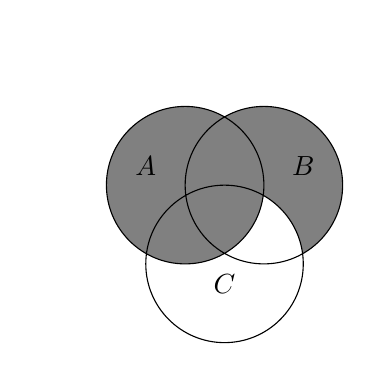
\begin{tikzpicture}[fill=gray]
    \scope
    \clip (-2,-2) rectangle (2,2)
    (0.5,-1) circle (1);
    \fill (1,0) circle (1);
    \endscope
    \fill (0,0) circle (1);
    \draw (0,0) circle (1) (-0.5,0) node [text=black,above] {$A$}
    (1,0) circle (1) (1.5, 0) node [text=black,above] {$B$}
    (0.5,-1) circle (1) (0.5,-1.5) node [text=black,above] {$C$};
  \end{tikzpicture}
  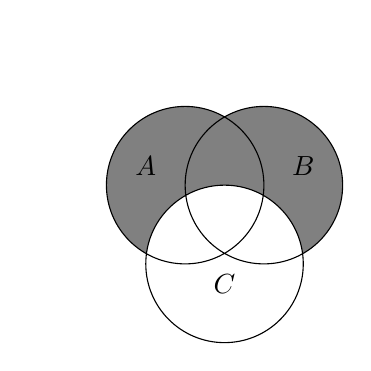
\begin{tikzpicture}[fill=gray]
    \scope
    \clip (-2,-2) rectangle (2,2)
    (0.5,-1) circle (1);
    \fill (0,0) circle (1)
    (1,0) circle (1);
    \endscope
    \draw (0,0) circle (1) (-0.5,0) node [text=black,above] {$A$}
    (1,0) circle (1) (1.5, 0) node [text=black,above] {$B$}
    (0.5,-1) circle (1) (0.5,-1.5) node [text=black,above] {$C$};
  \end{tikzpicture}

  From the pictures, we can conclude that $(A \cup B) \setminus C \subset A \cup (B \setminus C)$.
\item
  Let $A = \{1,4,5,7\}, B = \{2,4,6,7\}, C = \{3,5,6,7\}$, then $A \cup (B \setminus C) = \{1,2,4,5,7\}$ and $(A \cup B) \setminus C = \{1,2,4\}$.
  \end{enumerate}
  \pagebreak
\item
  \begin{enumerate}
    \item
  $B \triangle C$, and $A \triangle (B \triangle C)$:

  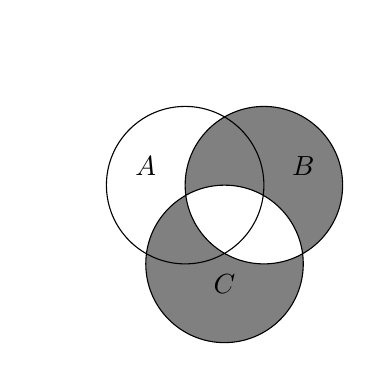
\begin{tikzpicture}[fill=gray]
    \scope
    \clip (-2,-2) rectangle (2,2)
    (1,0) circle (1);
    \fill (0.5,-1) circle (1);
    \endscope
    \scope
    \clip (-2,-2) rectangle (2,2)
    (0.5,-1) circle (1);
    \fill (1,0) circle (1);
    \endscope
    \draw (0,0) circle (1) (-0.5,0) node [text=black,above] {$A$}
    (1,0) circle (1) (1.5, 0) node [text=black,above] {$B$}
    (0.5,-1) circle (1) (0.5,-1.5) node [text=black,above] {$C$};
  \end{tikzpicture}
    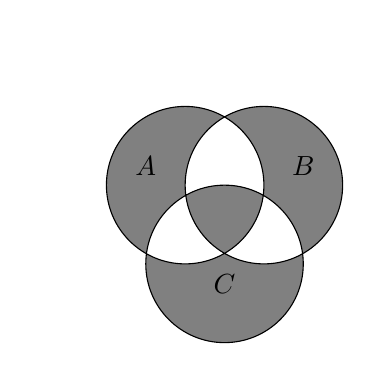
\begin{tikzpicture}[fill=gray]
    \scope
    \clip
    (0,0) circle (1)
    (0.5,-1) circle (1)
     (-2,-2) rectangle (2,2);
    \fill (1,0) circle (1);
    \endscope
    \scope
    \clip(1,0) circle (1)
    (0.5,-1) circle (1)
    (-2,-2) rectangle (2,2);
    \fill (0,0) circle (1);
    \endscope
    \scope
    \clip(1,0) circle (1)
    (0,0) circle (1)
    (-2,-2) rectangle (2,2);
    \fill (0.5,-1) circle (1);
    \endscope
    \draw (0,0) circle (1) (-0.5,0) node [text=black,above] {$A$}
    (1,0) circle (1) (1.5, 0) node [text=black,above] {$B$}
    (0.5,-1) circle (1) (0.5,-1.5) node [text=black,above] {$C$};
    \end{tikzpicture}

  \item
    $A \triangle B$ and $(A \triangle B) \triangle C$:

  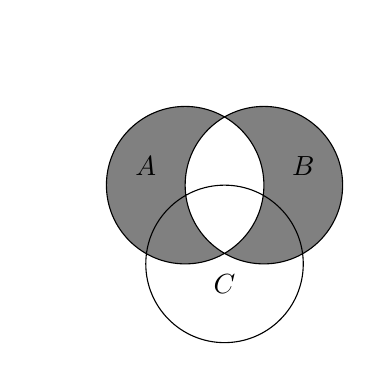
\begin{tikzpicture}[fill=gray]
    \scope
    \clip (-2,-2) rectangle (2,2)
    (0,0) circle (1);
    \fill (1,0) circle (1);
    \endscope
    \scope
    \clip (-2,-2) rectangle (2,2)
    (1,0) circle (1);
    \fill (0,0) circle (1);
    \endscope
    \draw (0,0) circle (1) (-0.5,0) node [text=black,above] {$A$}
    (1,0) circle (1) (1.5, 0) node [text=black,above] {$B$}
    (0.5,-1) circle (1) (0.5,-1.5) node [text=black,above] {$C$};
  \end{tikzpicture}
    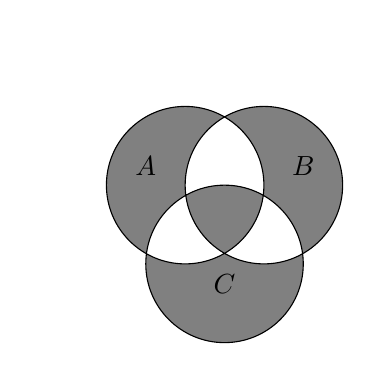
\begin{tikzpicture}[fill=gray]
    \scope
    \clip
    (0,0) circle (1)
    (0.5,-1) circle (1)
     (-2,-2) rectangle (2,2);
    \fill (1,0) circle (1);
    \endscope
    \scope
    \clip(1,0) circle (1)
    (0.5,-1) circle (1)
    (-2,-2) rectangle (2,2);
    \fill (0,0) circle (1);
    \endscope
    \scope
    \clip(1,0) circle (1)
    (0,0) circle (1)
    (-2,-2) rectangle (2,2);
    \fill (0.5,-1) circle (1);
    \endscope
    \draw (0,0) circle (1) (-0.5,0) node [text=black,above] {$A$}
    (1,0) circle (1) (1.5, 0) node [text=black,above] {$B$}
    (0.5,-1) circle (1) (0.5,-1.5) node [text=black,above] {$C$};
    \end{tikzpicture}

    Based on the diagrams, we can conclude that $A \triangle (B \triangle C) = (A \triangle B) \triangle C$.

  \end{enumerate}
\end{enumerate}
\section*{1.5 Exercises}
\begin{enumerate}
\item
  \begin{enumerate}
  \item $(S \lor \lnot E) \Rightarrow \lnot H$

    Where $S$ stands for ``Gas has unpleasant smell'', $E$ stands for ``Gas is explosive'' and $H$ stands for ``Gas is hydrogen''.

  \item $(F \land H) \Rightarrow D$

    Where $F$ stands for ``George has a fever'', $H$ stands for ``George has a headache'', and $D$ stands for ``George sees the doctor''.

  \item $(F \Rightarrow D) \land (H \Rightarrow D)$
  \item $(x \neq 2) \Rightarrow (P(x) \Rightarrow O(x))$

    Where $P(x)$ means ``$x$ is prime'', and $O(x)$ means ``$x$ is odd''.
  \end{enumerate}
\item
  \begin{enumerate}
  \item $(P \land A) \Rightarrow S$

    Where $P$ stands for ``Mary gets a good price'', $A$ stands for ``Mary finds a nice apartment'', and $S$ stands for ``Mary sells her house''.

  \item $(H \land D) \Rightarrow M$

    Where $H$ stands for ``You have a good credit history'', and $D$ stands for ``You have an adequate down payment'', and $M$ stands for ``You have a good mortgage''.

  \item $\lnot S \Rightarrow K$

    Where $S$ stands for ``Someone stops John'', and $K$ stands for ``John kills himself''.

  \item $(D(x,4) \lor D(x,6)) \Rightarrow \lnot P(x)$

    Where $D(x,y)$ means ``$x$ is divisible by $y$'', and $P(x)$ means ``$x$ is prime''.
  \end{enumerate}
\item
  \begin{enumerate}
\item $R \Rightarrow (W \land \lnot S)$

    Where $R$ stands for ``It is raining'', $W$ stands for ``It is windy'', and $S$ stands for ``The sun is shining''.

  \item $\lnot (W \land \lnot S) \Rightarrow \lnot R$.

    This is the contrapositive of (a), so they're equivalent.

  \item $R \Rightarrow (W \land \lnot S)$

    This is equivalent to (a).

  \item $(W \land \lnot S) \Rightarrow R$

    This is equivalent to the converse of (a).

  \item $(S \lor \lnot W) \Rightarrow \lnot R \equiv \lnot (W \land \lnot S) \Rightarrow \lnot R$

    This is the contrapositive of (a), meaning it is also equivalent to (a).

  \item
    \begin{equation*}
      \begin{aligned}
        (\lnot W \Rightarrow \lnot R) \land (\lnot \lnot S \Rightarrow \lnot R) &\equiv (R \Rightarrow W) \land (R \Rightarrow \lnot S) \\
        &\equiv (\lnot R \lor W) \land (\lnot R \lor \lnot S) \\
        &\equiv \lnot R \lor (W \land \lnot S) \\
        &\equiv R \Rightarrow (W \land \lnot S)
      \end{aligned}
    \end{equation*}

    This shows that it is equivalent to (a).
  \item
    \begin{equation*}
      \begin{aligned}
        (\lnot R \Rightarrow \lnot W) \lor (\lnot R \Rightarrow \lnot \lnot S) &\equiv (\lnot \lnot R \lor \lnot W) \lor (\lnot \lnot R \lor \lnot \lnot S) \\
        &\equiv (R \lor \lnot W) \lor (R \lor S) \\
        &\equiv \lnot W \lor S \lor R \\
        &\equiv (\lnot W \lor S) \lor R \\
        &\equiv \lnot (W \land \lnot S) \lor R \\
        &\equiv (W \land \lnot S) \Rightarrow R
      \end{aligned}
    \end{equation*}

    This shows that this statement is equivalent to the converse of (a).
  \end{enumerate}

\item
  \begin{enumerate}
  \item
    Let $S$ stand for ``Sales will go up'', $E$ stand for ``Expenses will go up'', and $H$ stand for ``The boss will be happy''.

    The premises are: $S \lor E$, $S \Rightarrow H$, $E \Rightarrow \lnot H$.  We'll rewrite the two conditionals as $\lnot S \lor H$ and $\lnot E \lor \lnot H$.

    The conclusion is $\lnot (S \lor E)$.

    \begin{tabular}{c c c c}
      $S \lor E$ & $\lnot S \lor H$ & $\lnot E \lor \lnot H$ & $\lnot (S \land E)$ \\ \hline
      T & T & F & F \\
      T & F & T & F \\
      T & T & T & T \\
      T & F & T & T \\
      T & T & F & T \\
      T & T & T & T \\
      F & T & T & T \\
      F & T & T & T \\
    \end{tabular}

    Rows 2 and 6 are where all 3 premises are true, and so is the conclusion so this argument is valid.

  \item
    Let $T$ stand for ``Taxes will go up'', $U$ stand for ``Unemployment rate will go up'', $G$ stand for ``GNP will go up'', and $R$ stand for ``There will be a recession''.

    The premises are: $(T \land U) \Rightarrow R$, $G \Rightarrow \lnot R$, $G \land T$.

    The conclusion is $\lnot U$.

    We will rewrite the two conditional premises as $\lnot (T \land U) \lor R$, and $\lnot G \lor \lnot R$.

    \pagebreak

    The truth table is:

    \begin{tabular}{c c c c}
      $\lnot (T \land U) \lor R$ & $\lnot G \lor \lnot R$ & $G \land T$ & $\lnot U$ \\ \hline
      T & F & T & F \\
      F & T & T & F \\
      T & T & F & F \\
      F & T & F & F \\
      T & F & T & T \\
      T & T & T & T \\
      T & T & F & T \\
      T & T & F & T \\
      T & F & F & F \\
      T & T & F & F \\
      T & T & F & F \\
      T & T & F & F \\
      T & T & F & T \\
      T & T & F & T \\
      T & T & F & T \\
      T & T & F & T \\
    \end{tabular}

    The only row that all three premises are true is on line 6, and the conclusion is also true, so this argument is valid.

  \item
    Let $W$ stand for ``The warning light is on'', $P$ stand for ``Pressure is too high'', and $C$ stand for ``The relief valve is clogged.''

    The premises are $W \iff (P \land C)$ and $\lnot C$.

    We can rewrite the first premise as
    \begin{equation*}
      (W \Rightarrow (P \land C)) \land ((P \land C) \Rightarrow W) \equiv (\lnot W \lor (P \land C)) \land (\lnot (P \land C) \lor W)
    \end{equation*}

    The conclusion is $W \iff P$. We will rewrite this as

    \begin{equation*}
      (\lnot W \lor P) \land (\lnot P \lor W)
    \end{equation*}

    The truth table:

    \begin{tabular}{c c c}
      $(\lnot W \lor (P \land C)) \land (\lnot (P \land C) \lor W)$ &
      $\lnot C$ &
      $(\lnot W \lor P) \land (\lnot P \lor W)$ \\ \hline
      T & F & T \\
      F & T & T \\
      F & F & F \\
      F & T & F \\
      F & F & F \\
      T & T & F \\
      T & F & T \\
      T & T & T \\
    \end{tabular}

    This argument is not valid since both premises are true on line 6, but the conclusion is false.
  \end{enumerate}
\item
  \begin{enumerate}
  \item
    \begin{equation*}
      \begin{aligned}
        P \iff Q &\equiv (P \Rightarrow Q) \land (Q \Rightarrow P) & \text{Def. of biconditional} \\
        &\equiv (P \Rightarrow Q) \land (\lnot P \Rightarrow \lnot Q) & \text{Contrapositive} \\
        &\equiv (\lnot P \lor Q) \land (\lnot \lnot P \lor \lnot Q) \\
        &\equiv (\lnot P \lor Q) \land (P \lor \lnot Q) & \text{Double negation law} \\
        &\equiv ((\lnot P \lor Q) \land P) \lor ((\lnot P \lor Q) \land \lnot Q) & \text{Distributive law} \\
        &\equiv ((\lnot P \land P) \lor (P \land Q)) \lor ((\lnot P \land \lnot Q) \lor (Q \land \lnot Q)) & \text{Distributive law} \\
        &\equiv (P \land Q) \lor (\lnot P \land \lnot Q) & \text{Contradiction}
      \end{aligned}
    \end{equation*}

  \item
    \begin{equation*}
      \begin{aligned}
        (P \Rightarrow Q) \lor (P \Rightarrow R) &\equiv (\lnot P \lor Q) \lor (\lnot P \lor R) \\
        &\equiv \lnot P \lor Q \lor \lnot P \lor R & \text{Associative law} \\
        &\equiv \lnot P \lor Q \lor R \\
        &\equiv \lnot P \lor (Q \lor R) & \text{Associative law} \\
        &\equiv P \Rightarrow (Q \lor R)
      \end{aligned}
    \end{equation*}
  \end{enumerate}
\item
  \begin{enumerate}
  \item
    \begin{equation*}
      \begin{aligned}
        (P \Rightarrow R) \land (Q \Rightarrow R) &\equiv (\lnot P \lor R) \land (\lnot Q \lor R) \\
        &\equiv (\lnot P \land \lnot Q) \lor R & \text{Distributive law} \\
        &\equiv \lnot (P \lor Q) \lor R & \text{DeMorgan's law} \\
        &\equiv (P \lor Q) \Rightarrow R
      \end{aligned}
    \end{equation*}
  \item
     \begin{equation*}
       \begin{aligned}
         (P \Rightarrow R) \lor (Q \Rightarrow R) &\equiv (\lnot P \lor R) \lor (\lnot Q \lor R) \\
         &\equiv \lnot P \lor R \lor \lnot Q \lor R & \text{Associative law} \\
         &\equiv \lnot P \lor R \lor \lnot Q \\
         &\equiv \lnot P \lor \lnot Q \lor R & \text{Commutative law} \\
         &\equiv (\lnot P \lor \lnot Q) \lor R & \text{Associative law} \\
         &\equiv \lnot (P \land Q) \lor R & \text{DeMorgan's law} \\
         &\equiv (P \land Q) \Rightarrow R
       \end{aligned}
    \end{equation*}

     This shows that $(P \Rightarrow R) \lor (Q \Rightarrow R) \equiv (P \land Q) \Rightarrow R$.
  \end{enumerate}

\item
  \begin{enumerate}
    \item
      We can demonstrate this using a truth table.  To save space, I'll only show the truth tables of the two expressions without the intermediate steps:

      \begin{tabular}{c c}
        $(P \Rightarrow Q) \land (Q \Rightarrow R)$ & $(P \Rightarrow R) \land [(P \iff Q) \lor (R \iff Q)]$ \\ \hline
        T & T \\
        F & F \\
        F & F \\
        F & F \\
        T & T \\
        F & F \\
        T & T \\
        T & T \\
      \end{tabular}
    \item
      Again, we can use a truth table:

      \begin{tabular}{c c c}
        $(P \Rightarrow Q)$ & $(Q \Rightarrow R)$ & $(P \Rightarrow Q) \lor (Q \Rightarrow R)$ \\ \hline
        T & T & T \\
        T & F & T \\
        F & T & T \\
        F & T & T \\
        T & T & T \\
        T & F & T \\
        T & T & T \\
        T & T & T \\
      \end{tabular}
  \end{enumerate}
\item
  We know that $(P \Rightarrow Q) \equiv (\lnot P \lor Q)$.  By negating the expression, we have $\lnot (\lnot P \lor Q) \equiv P \land \lnot Q$.  We just need to get rid of the $\lnot$, and we can do that by \starting off with $\lnot Q$:
  \begin{equation*}
    \begin{aligned}
      $\not (P \Rightarrow \lnot Q) &\equiv \lnot (\lnot P \lor \lnot Q) \\
      &\equiv \lnot \lnot P \land \lnot \lnot Q \\
      &\equiv P \land Q
    \end{aligned}
    \end{equation*}
\item
  We know that $(P \iff Q) \equiv (P \Rightarrow Q) \land (Q \Rightarrow P)$.  From problem 8, we already know how to find the equivalent of $\land$ using only $\lnot$ and $\Rightarrow$, so $\iff$ is equivalent to $\lnot [(P \Rightarrow Q) \Rightarrow \lnot (Q \Rightarrow P)]$.
\item
  (a), (b), and (d) are equivalent because they're all equivalent to $\lnot P \lor \lnot Q \lor R$.  (e) and (c) are equivalent because they're both equivalent to $(\lnot P \lor Q) \land (\lnot P \lor R)$.
\end{enumerate}
\end{document}
